\section{符号约定}
该手册对数据结构格式,指令的符号表示以及十六进制和二进制数使用的表示方法如下所述。
\subsection{比特和字节顺序}
在存储器中的数据结构的图示中,较小的地址出现在图的底部;地址增加到顶部。比特位置从右到左编号。一个特定比特的数值等于 2 的比特位置次方。英特尔 64 和 IA-32 处理器是“小端”机器;这意味着字的字节从最低有效字节开始编号。见 \autoref{fig:1-1}。
\begin{figure}[H]
\centering
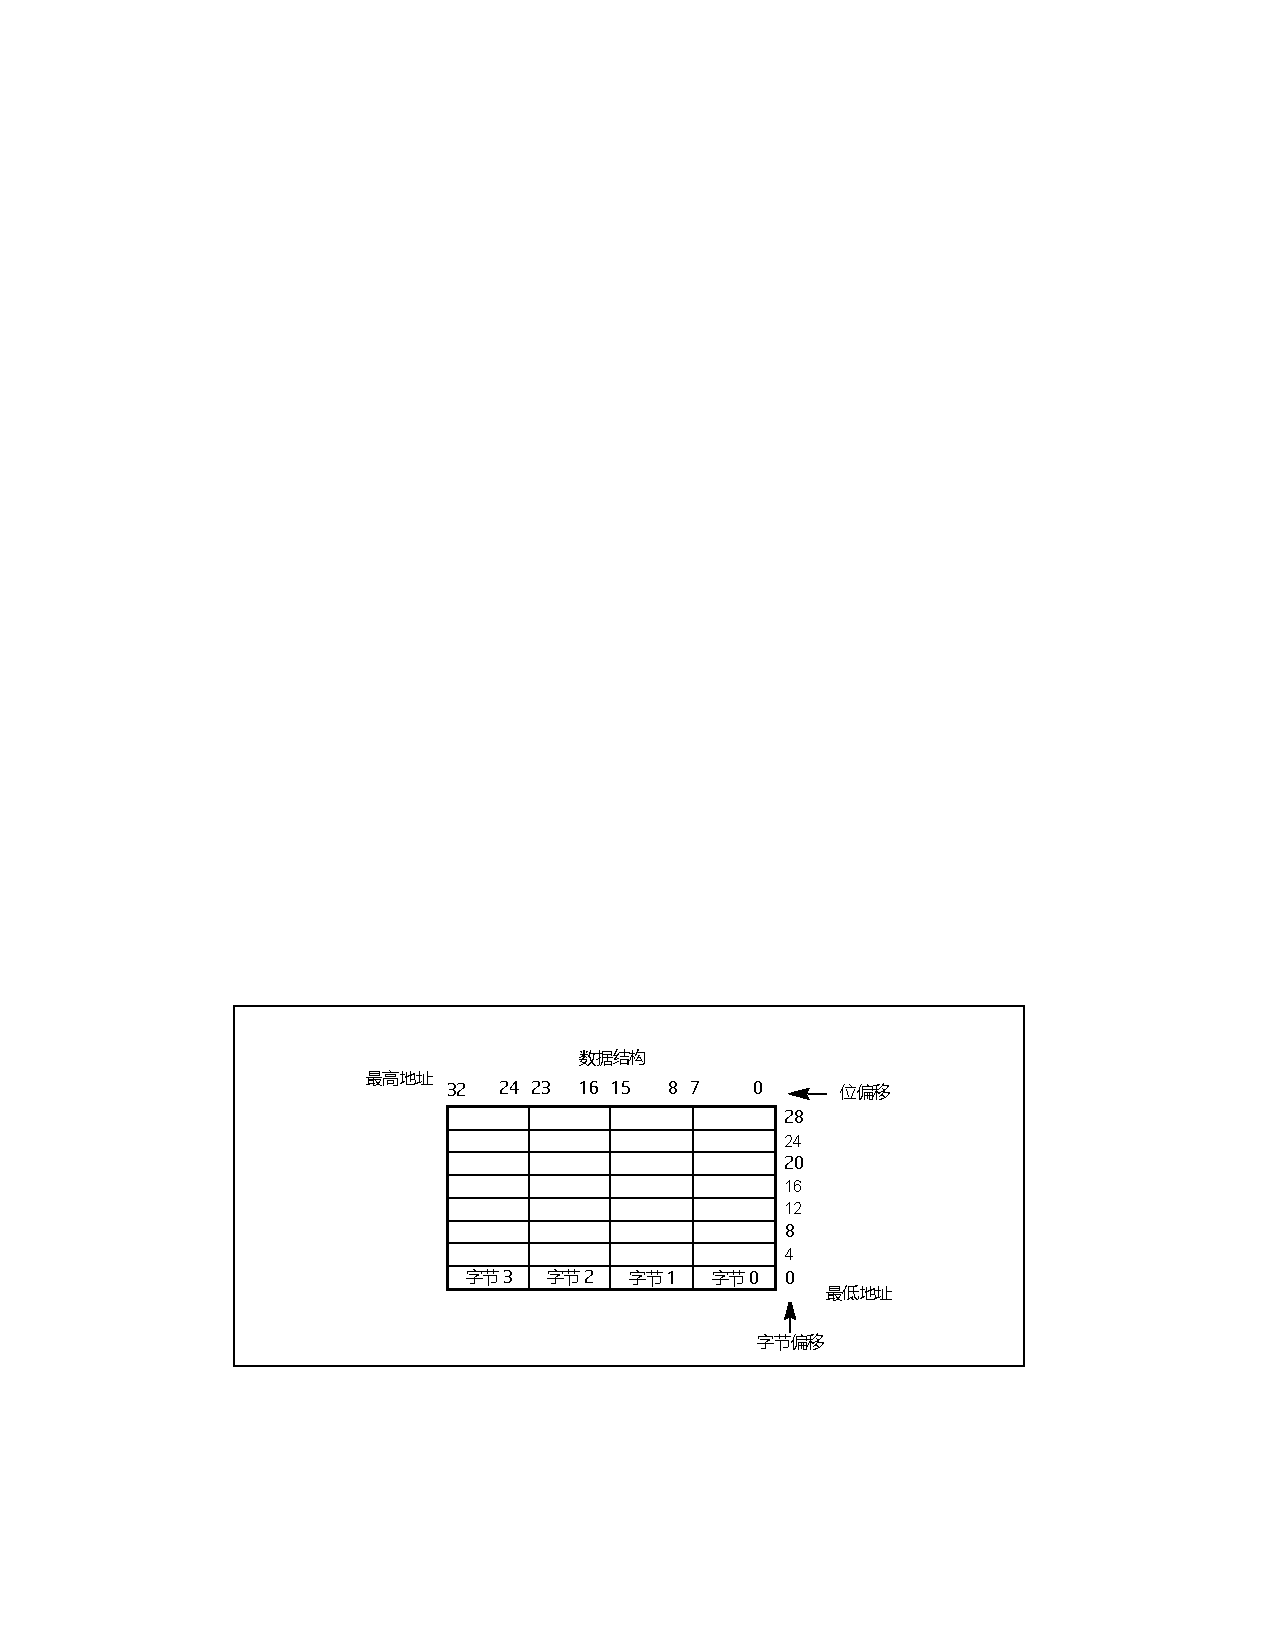
\includegraphics[scale=1]{1-1.pdf}
\caption{位和字节顺序}
\label{fig:1-1}
\end{figure}

\subsection{保留位和软件兼容性}
在许多寄存器和内存分布描述中,一些特定的位被标记为